\documentclass[11pt,a4paper]{article}
\usepackage[spanish,es-nodecimaldot]{babel}	% Utilizar español
\usepackage[utf8]{inputenc}					% Caracteres UTF-8
\usepackage{graphicx}						% Imagenes
\usepackage[hidelinks]{hyperref}			% Poner enlaces sin marcarlos en rojo
\usepackage{fancyhdr}						% Modificar encabezados y pies de pagina
\usepackage{float}							% Insertar figuras
\usepackage[textwidth=400pt]{geometry}		% Anchura de la pagina
\usepackage[nottoc]{tocbibind}				% Referencias (no incluir num pagina indice en Indice)
\usepackage{enumitem}						% Permitir enumerate con distintos simbolos
\usepackage[T1]{fontenc}					% Usar textsc en sections
\usepackage{amsmath}						% Símbolos matemáticos
\usepackage{fancyvrb} % verbatim replacement that allows latex
\usepackage{upquote} % Upright quotes for verbatim code
\usepackage{xcolor}


% Comando para poner el nombre de la asignatura
\newcommand{\asignatura}{Aprendizaje Automático}
\newcommand{\autor}{Vladislav Nikolov Vasilev}

% Configuracion de encabezados y pies de pagina
\pagestyle{fancy}
\lhead{\autor{}}
\rhead{\asignatura{}}
\lfoot{Grado en Ingeniería Informática}
\cfoot{}
\rfoot{\thepage}
\renewcommand{\headrulewidth}{0.4pt}		% Linea cabeza de pagina
\renewcommand{\footrulewidth}{0.4pt}		% Linea pie de pagina


    % Colors for the hyperref package
    \definecolor{urlcolor}{rgb}{0,.145,.698}
    \definecolor{linkcolor}{rgb}{.71,0.21,0.01}
    \definecolor{citecolor}{rgb}{.12,.54,.11}

    % ANSI colors
    \definecolor{ansi-black}{HTML}{3E424D}
    \definecolor{ansi-black-intense}{HTML}{282C36}
    \definecolor{ansi-red}{HTML}{E75C58}
    \definecolor{ansi-red-intense}{HTML}{B22B31}
    \definecolor{ansi-green}{HTML}{00A250}
    \definecolor{ansi-green-intense}{HTML}{007427}
    \definecolor{ansi-yellow}{HTML}{DDB62B}
    \definecolor{ansi-yellow-intense}{HTML}{B27D12}
    \definecolor{ansi-blue}{HTML}{208FFB}
    \definecolor{ansi-blue-intense}{HTML}{0065CA}
    \definecolor{ansi-magenta}{HTML}{D160C4}
    \definecolor{ansi-magenta-intense}{HTML}{A03196}
    \definecolor{ansi-cyan}{HTML}{60C6C8}
    \definecolor{ansi-cyan-intense}{HTML}{258F8F}
    \definecolor{ansi-white}{HTML}{C5C1B4}
    \definecolor{ansi-white-intense}{HTML}{A1A6B2}
    \definecolor{ansi-default-inverse-fg}{HTML}{FFFFFF}
    \definecolor{ansi-default-inverse-bg}{HTML}{000000}

    % commands and environments needed by pandoc snippets
    % extracted from the output of `pandoc -s`
    \providecommand{\tightlist}{%
      \setlength{\itemsep}{0pt}\setlength{\parskip}{0pt}}
    \DefineVerbatimEnvironment{Highlighting}{Verbatim}{commandchars=\\\{\}}
    % Add ',fontsize=\small' for more characters per line
    \newenvironment{Shaded}{}{}
    \newcommand{\KeywordTok}[1]{\textcolor[rgb]{0.00,0.44,0.13}{\textbf{{#1}}}}
    \newcommand{\DataTypeTok}[1]{\textcolor[rgb]{0.56,0.13,0.00}{{#1}}}
    \newcommand{\DecValTok}[1]{\textcolor[rgb]{0.25,0.63,0.44}{{#1}}}
    \newcommand{\BaseNTok}[1]{\textcolor[rgb]{0.25,0.63,0.44}{{#1}}}
    \newcommand{\FloatTok}[1]{\textcolor[rgb]{0.25,0.63,0.44}{{#1}}}
    \newcommand{\CharTok}[1]{\textcolor[rgb]{0.25,0.44,0.63}{{#1}}}
    \newcommand{\StringTok}[1]{\textcolor[rgb]{0.25,0.44,0.63}{{#1}}}
    \newcommand{\CommentTok}[1]{\textcolor[rgb]{0.38,0.63,0.69}{\textit{{#1}}}}
    \newcommand{\OtherTok}[1]{\textcolor[rgb]{0.00,0.44,0.13}{{#1}}}
    \newcommand{\AlertTok}[1]{\textcolor[rgb]{1.00,0.00,0.00}{\textbf{{#1}}}}
    \newcommand{\FunctionTok}[1]{\textcolor[rgb]{0.02,0.16,0.49}{{#1}}}
    \newcommand{\RegionMarkerTok}[1]{{#1}}
    \newcommand{\ErrorTok}[1]{\textcolor[rgb]{1.00,0.00,0.00}{\textbf{{#1}}}}
    \newcommand{\NormalTok}[1]{{#1}}
    
    % Additional commands for more recent versions of Pandoc
    \newcommand{\ConstantTok}[1]{\textcolor[rgb]{0.53,0.00,0.00}{{#1}}}
    \newcommand{\SpecialCharTok}[1]{\textcolor[rgb]{0.25,0.44,0.63}{{#1}}}
    \newcommand{\VerbatimStringTok}[1]{\textcolor[rgb]{0.25,0.44,0.63}{{#1}}}
    \newcommand{\SpecialStringTok}[1]{\textcolor[rgb]{0.73,0.40,0.53}{{#1}}}
    \newcommand{\ImportTok}[1]{{#1}}
    \newcommand{\DocumentationTok}[1]{\textcolor[rgb]{0.73,0.13,0.13}{\textit{{#1}}}}
    \newcommand{\AnnotationTok}[1]{\textcolor[rgb]{0.38,0.63,0.69}{\textbf{\textit{{#1}}}}}
    \newcommand{\CommentVarTok}[1]{\textcolor[rgb]{0.38,0.63,0.69}{\textbf{\textit{{#1}}}}}
    \newcommand{\VariableTok}[1]{\textcolor[rgb]{0.10,0.09,0.49}{{#1}}}
    \newcommand{\ControlFlowTok}[1]{\textcolor[rgb]{0.00,0.44,0.13}{\textbf{{#1}}}}
    \newcommand{\OperatorTok}[1]{\textcolor[rgb]{0.40,0.40,0.40}{{#1}}}
    \newcommand{\BuiltInTok}[1]{{#1}}
    \newcommand{\ExtensionTok}[1]{{#1}}
    \newcommand{\PreprocessorTok}[1]{\textcolor[rgb]{0.74,0.48,0.00}{{#1}}}
    \newcommand{\AttributeTok}[1]{\textcolor[rgb]{0.49,0.56,0.16}{{#1}}}
    \newcommand{\InformationTok}[1]{\textcolor[rgb]{0.38,0.63,0.69}{\textbf{\textit{{#1}}}}}
    \newcommand{\WarningTok}[1]{\textcolor[rgb]{0.38,0.63,0.69}{\textbf{\textit{{#1}}}}}
    
    
    % Define a nice break command that doesn't care if a line doesn't already
    % exist.
    \def\br{\hspace*{\fill} \\* }
    % Math Jax compatibility definitions
    \def\gt{>}
    \def\lt{<}
    \let\Oldtex\TeX
    \let\Oldlatex\LaTeX
    \renewcommand{\TeX}{\textrm{\Oldtex}}
    \renewcommand{\LaTeX}{\textrm{\Oldlatex}}
    % Document parameters
    % Document title
    \title{memoria}
    
    
    
    
    

    % Pygments definitions
    
\makeatletter
\def\PY@reset{\let\PY@it=\relax \let\PY@bf=\relax%
    \let\PY@ul=\relax \let\PY@tc=\relax%
    \let\PY@bc=\relax \let\PY@ff=\relax}
\def\PY@tok#1{\csname PY@tok@#1\endcsname}
\def\PY@toks#1+{\ifx\relax#1\empty\else%
    \PY@tok{#1}\expandafter\PY@toks\fi}
\def\PY@do#1{\PY@bc{\PY@tc{\PY@ul{%
    \PY@it{\PY@bf{\PY@ff{#1}}}}}}}
\def\PY#1#2{\PY@reset\PY@toks#1+\relax+\PY@do{#2}}

\expandafter\def\csname PY@tok@w\endcsname{\def\PY@tc##1{\textcolor[rgb]{0.73,0.73,0.73}{##1}}}
\expandafter\def\csname PY@tok@c\endcsname{\let\PY@it=\textit\def\PY@tc##1{\textcolor[rgb]{0.25,0.50,0.50}{##1}}}
\expandafter\def\csname PY@tok@cp\endcsname{\def\PY@tc##1{\textcolor[rgb]{0.74,0.48,0.00}{##1}}}
\expandafter\def\csname PY@tok@k\endcsname{\let\PY@bf=\textbf\def\PY@tc##1{\textcolor[rgb]{0.00,0.50,0.00}{##1}}}
\expandafter\def\csname PY@tok@kp\endcsname{\def\PY@tc##1{\textcolor[rgb]{0.00,0.50,0.00}{##1}}}
\expandafter\def\csname PY@tok@kt\endcsname{\def\PY@tc##1{\textcolor[rgb]{0.69,0.00,0.25}{##1}}}
\expandafter\def\csname PY@tok@o\endcsname{\def\PY@tc##1{\textcolor[rgb]{0.40,0.40,0.40}{##1}}}
\expandafter\def\csname PY@tok@ow\endcsname{\let\PY@bf=\textbf\def\PY@tc##1{\textcolor[rgb]{0.67,0.13,1.00}{##1}}}
\expandafter\def\csname PY@tok@nb\endcsname{\def\PY@tc##1{\textcolor[rgb]{0.00,0.50,0.00}{##1}}}
\expandafter\def\csname PY@tok@nf\endcsname{\def\PY@tc##1{\textcolor[rgb]{0.00,0.00,1.00}{##1}}}
\expandafter\def\csname PY@tok@nc\endcsname{\let\PY@bf=\textbf\def\PY@tc##1{\textcolor[rgb]{0.00,0.00,1.00}{##1}}}
\expandafter\def\csname PY@tok@nn\endcsname{\let\PY@bf=\textbf\def\PY@tc##1{\textcolor[rgb]{0.00,0.00,1.00}{##1}}}
\expandafter\def\csname PY@tok@ne\endcsname{\let\PY@bf=\textbf\def\PY@tc##1{\textcolor[rgb]{0.82,0.25,0.23}{##1}}}
\expandafter\def\csname PY@tok@nv\endcsname{\def\PY@tc##1{\textcolor[rgb]{0.10,0.09,0.49}{##1}}}
\expandafter\def\csname PY@tok@no\endcsname{\def\PY@tc##1{\textcolor[rgb]{0.53,0.00,0.00}{##1}}}
\expandafter\def\csname PY@tok@nl\endcsname{\def\PY@tc##1{\textcolor[rgb]{0.63,0.63,0.00}{##1}}}
\expandafter\def\csname PY@tok@ni\endcsname{\let\PY@bf=\textbf\def\PY@tc##1{\textcolor[rgb]{0.60,0.60,0.60}{##1}}}
\expandafter\def\csname PY@tok@na\endcsname{\def\PY@tc##1{\textcolor[rgb]{0.49,0.56,0.16}{##1}}}
\expandafter\def\csname PY@tok@nt\endcsname{\let\PY@bf=\textbf\def\PY@tc##1{\textcolor[rgb]{0.00,0.50,0.00}{##1}}}
\expandafter\def\csname PY@tok@nd\endcsname{\def\PY@tc##1{\textcolor[rgb]{0.67,0.13,1.00}{##1}}}
\expandafter\def\csname PY@tok@s\endcsname{\def\PY@tc##1{\textcolor[rgb]{0.73,0.13,0.13}{##1}}}
\expandafter\def\csname PY@tok@sd\endcsname{\let\PY@it=\textit\def\PY@tc##1{\textcolor[rgb]{0.73,0.13,0.13}{##1}}}
\expandafter\def\csname PY@tok@si\endcsname{\let\PY@bf=\textbf\def\PY@tc##1{\textcolor[rgb]{0.73,0.40,0.53}{##1}}}
\expandafter\def\csname PY@tok@se\endcsname{\let\PY@bf=\textbf\def\PY@tc##1{\textcolor[rgb]{0.73,0.40,0.13}{##1}}}
\expandafter\def\csname PY@tok@sr\endcsname{\def\PY@tc##1{\textcolor[rgb]{0.73,0.40,0.53}{##1}}}
\expandafter\def\csname PY@tok@ss\endcsname{\def\PY@tc##1{\textcolor[rgb]{0.10,0.09,0.49}{##1}}}
\expandafter\def\csname PY@tok@sx\endcsname{\def\PY@tc##1{\textcolor[rgb]{0.00,0.50,0.00}{##1}}}
\expandafter\def\csname PY@tok@m\endcsname{\def\PY@tc##1{\textcolor[rgb]{0.40,0.40,0.40}{##1}}}
\expandafter\def\csname PY@tok@gh\endcsname{\let\PY@bf=\textbf\def\PY@tc##1{\textcolor[rgb]{0.00,0.00,0.50}{##1}}}
\expandafter\def\csname PY@tok@gu\endcsname{\let\PY@bf=\textbf\def\PY@tc##1{\textcolor[rgb]{0.50,0.00,0.50}{##1}}}
\expandafter\def\csname PY@tok@gd\endcsname{\def\PY@tc##1{\textcolor[rgb]{0.63,0.00,0.00}{##1}}}
\expandafter\def\csname PY@tok@gi\endcsname{\def\PY@tc##1{\textcolor[rgb]{0.00,0.63,0.00}{##1}}}
\expandafter\def\csname PY@tok@gr\endcsname{\def\PY@tc##1{\textcolor[rgb]{1.00,0.00,0.00}{##1}}}
\expandafter\def\csname PY@tok@ge\endcsname{\let\PY@it=\textit}
\expandafter\def\csname PY@tok@gs\endcsname{\let\PY@bf=\textbf}
\expandafter\def\csname PY@tok@gp\endcsname{\let\PY@bf=\textbf\def\PY@tc##1{\textcolor[rgb]{0.00,0.00,0.50}{##1}}}
\expandafter\def\csname PY@tok@go\endcsname{\def\PY@tc##1{\textcolor[rgb]{0.53,0.53,0.53}{##1}}}
\expandafter\def\csname PY@tok@gt\endcsname{\def\PY@tc##1{\textcolor[rgb]{0.00,0.27,0.87}{##1}}}
\expandafter\def\csname PY@tok@err\endcsname{\def\PY@bc##1{\setlength{\fboxsep}{0pt}\fcolorbox[rgb]{1.00,0.00,0.00}{1,1,1}{\strut ##1}}}
\expandafter\def\csname PY@tok@kc\endcsname{\let\PY@bf=\textbf\def\PY@tc##1{\textcolor[rgb]{0.00,0.50,0.00}{##1}}}
\expandafter\def\csname PY@tok@kd\endcsname{\let\PY@bf=\textbf\def\PY@tc##1{\textcolor[rgb]{0.00,0.50,0.00}{##1}}}
\expandafter\def\csname PY@tok@kn\endcsname{\let\PY@bf=\textbf\def\PY@tc##1{\textcolor[rgb]{0.00,0.50,0.00}{##1}}}
\expandafter\def\csname PY@tok@kr\endcsname{\let\PY@bf=\textbf\def\PY@tc##1{\textcolor[rgb]{0.00,0.50,0.00}{##1}}}
\expandafter\def\csname PY@tok@bp\endcsname{\def\PY@tc##1{\textcolor[rgb]{0.00,0.50,0.00}{##1}}}
\expandafter\def\csname PY@tok@fm\endcsname{\def\PY@tc##1{\textcolor[rgb]{0.00,0.00,1.00}{##1}}}
\expandafter\def\csname PY@tok@vc\endcsname{\def\PY@tc##1{\textcolor[rgb]{0.10,0.09,0.49}{##1}}}
\expandafter\def\csname PY@tok@vg\endcsname{\def\PY@tc##1{\textcolor[rgb]{0.10,0.09,0.49}{##1}}}
\expandafter\def\csname PY@tok@vi\endcsname{\def\PY@tc##1{\textcolor[rgb]{0.10,0.09,0.49}{##1}}}
\expandafter\def\csname PY@tok@vm\endcsname{\def\PY@tc##1{\textcolor[rgb]{0.10,0.09,0.49}{##1}}}
\expandafter\def\csname PY@tok@sa\endcsname{\def\PY@tc##1{\textcolor[rgb]{0.73,0.13,0.13}{##1}}}
\expandafter\def\csname PY@tok@sb\endcsname{\def\PY@tc##1{\textcolor[rgb]{0.73,0.13,0.13}{##1}}}
\expandafter\def\csname PY@tok@sc\endcsname{\def\PY@tc##1{\textcolor[rgb]{0.73,0.13,0.13}{##1}}}
\expandafter\def\csname PY@tok@dl\endcsname{\def\PY@tc##1{\textcolor[rgb]{0.73,0.13,0.13}{##1}}}
\expandafter\def\csname PY@tok@s2\endcsname{\def\PY@tc##1{\textcolor[rgb]{0.73,0.13,0.13}{##1}}}
\expandafter\def\csname PY@tok@sh\endcsname{\def\PY@tc##1{\textcolor[rgb]{0.73,0.13,0.13}{##1}}}
\expandafter\def\csname PY@tok@s1\endcsname{\def\PY@tc##1{\textcolor[rgb]{0.73,0.13,0.13}{##1}}}
\expandafter\def\csname PY@tok@mb\endcsname{\def\PY@tc##1{\textcolor[rgb]{0.40,0.40,0.40}{##1}}}
\expandafter\def\csname PY@tok@mf\endcsname{\def\PY@tc##1{\textcolor[rgb]{0.40,0.40,0.40}{##1}}}
\expandafter\def\csname PY@tok@mh\endcsname{\def\PY@tc##1{\textcolor[rgb]{0.40,0.40,0.40}{##1}}}
\expandafter\def\csname PY@tok@mi\endcsname{\def\PY@tc##1{\textcolor[rgb]{0.40,0.40,0.40}{##1}}}
\expandafter\def\csname PY@tok@il\endcsname{\def\PY@tc##1{\textcolor[rgb]{0.40,0.40,0.40}{##1}}}
\expandafter\def\csname PY@tok@mo\endcsname{\def\PY@tc##1{\textcolor[rgb]{0.40,0.40,0.40}{##1}}}
\expandafter\def\csname PY@tok@ch\endcsname{\let\PY@it=\textit\def\PY@tc##1{\textcolor[rgb]{0.25,0.50,0.50}{##1}}}
\expandafter\def\csname PY@tok@cm\endcsname{\let\PY@it=\textit\def\PY@tc##1{\textcolor[rgb]{0.25,0.50,0.50}{##1}}}
\expandafter\def\csname PY@tok@cpf\endcsname{\let\PY@it=\textit\def\PY@tc##1{\textcolor[rgb]{0.25,0.50,0.50}{##1}}}
\expandafter\def\csname PY@tok@c1\endcsname{\let\PY@it=\textit\def\PY@tc##1{\textcolor[rgb]{0.25,0.50,0.50}{##1}}}
\expandafter\def\csname PY@tok@cs\endcsname{\let\PY@it=\textit\def\PY@tc##1{\textcolor[rgb]{0.25,0.50,0.50}{##1}}}

\def\PYZbs{\char`\\}
\def\PYZus{\char`\_}
\def\PYZob{\char`\{}
\def\PYZcb{\char`\}}
\def\PYZca{\char`\^}
\def\PYZam{\char`\&}
\def\PYZlt{\char`\<}
\def\PYZgt{\char`\>}
\def\PYZsh{\char`\#}
\def\PYZpc{\char`\%}
\def\PYZdl{\char`\$}
\def\PYZhy{\char`\-}
\def\PYZsq{\char`\'}
\def\PYZdq{\char`\"}
\def\PYZti{\char`\~}
% for compatibility with earlier versions
\def\PYZat{@}
\def\PYZlb{[}
\def\PYZrb{]}
\makeatother


    % Exact colors from NB
    \definecolor{incolor}{rgb}{0.0, 0.0, 0.5}
    \definecolor{outcolor}{rgb}{0.545, 0.0, 0.0}

\begin{document}
\pagenumbering{gobble}

% Pagina de titulo
\begin{titlepage}

\begin{minipage}{\textwidth}

\centering


\includegraphics[scale=0.5]{img/ugr.png}\\

\textsc{\Large \asignatura{}\\[0.2cm]}
\textsc{GRADO EN INGENIERÍA INFORMÁTICA}\\[1cm]

\noindent\rule[-1ex]{\textwidth}{1pt}\\[1.5ex]
\textsc{{\Huge PRÁCTICA 3\\[0.5ex]}}
\textsc{{\Large Programación\\}}
\noindent\rule[-1ex]{\textwidth}{2pt}\\[3.5ex]

\end{minipage}

\vspace{0.5cm}

\begin{minipage}{\textwidth}

\centering

\textbf{Autor}\\ {\autor{}}\\[2.5ex]
\textbf{Rama}\\ {Computación y Sistemas Inteligentes}\\[2.5ex]
\vspace{0.3cm}


\includegraphics[scale=0.3]{img/etsiit.jpeg}

\vspace{0.7cm}
\textsc{Escuela Técnica Superior de Ingenierías Informática y de Telecomunicación}\\
\vspace{1cm}
\textsc{Curso 2018-2019}
\end{minipage}
\end{titlepage}

\pagenumbering{arabic}
\tableofcontents
\thispagestyle{empty}				% No usar estilo en la pagina de indice

\newpage

\setlength{\parskip}{1em}

\section{\textsc{Problema de Regresión}}

\subsection{Descripción del problema}

En este problema vamos a trabajar con el conjunto de datos \textit{Airfoil Self-Noise}, el cuál ha sido proporcionado por la NASA,
y contiene los resultados de haber realizado un conjunto de pruebas aerodinámicas y acústicas en un túnel de viento sobre perfiles
alares de dos y tres dimensiones.

El conjunto de datos está compuesto por 1503 filas y 6 columnas, los valores de las cuáles son todos números reales. Los datos de
las 5 primeras columnas se corresponden con los datos de entrada, y la última columna se corresponde con la información de salida.
A continuación se puede ver que representa cada uno de los atributos de forma ordenada:

\begin{enumerate}
	\item Frecuencia, medida en $Hz$.
	\item Ángulo de ataque (ángulo que forman la cuerda geométrica de un perfil alar con la dirección del aire incidente),
		  medida en grados.
	\item Longitud de la cuerda del perfil alar, medida en metros.
	\item Velocidad \textit{free-stream}, medida en metros por segundo. 
	\item Distancia de desplazamiento de succión, medida en metros.
	\item Nivel de presión sonora, medida en $dB$.
\end{enumerate}

 \subsection{Análisis de los datos}\label{anuxe1lisis-de-los-datos}

    Antes de comenzar con todo el proceso de elección y selección de un
modelo lineal, vamos a pararnos un momento para analizar los datos de
los que disponemos con el fin de obtener más información sobre el
problema.

Lo primero que tenemos que hacer es cargar los datos. Para ello, vamos a
usar una función genérica que nos permita leer ficheros de datos y
obtener un \emph{DataFrame} que podamos usar luego. Vamos a ver como
sería esta función:

\begin{Verbatim}[commandchars=\\\{\}]
{\color{incolor}In [{\color{incolor}1}]:} \PY{k+kn}{import} \PY{n+nn}{numpy} \PY{k}{as} \PY{n+nn}{np}
        \PY{k+kn}{import} \PY{n+nn}{pandas} \PY{k}{as} \PY{n+nn}{pd}
        \PY{k+kn}{import} \PY{n+nn}{matplotlib}\PY{n+nn}{.}\PY{n+nn}{pyplot} \PY{k}{as} \PY{n+nn}{plt}
        
        \PY{c+c1}{\PYZsh{} Establecer la semilla que vamos a utilizar}
        \PY{n}{np}\PY{o}{.}\PY{n}{random}\PY{o}{.}\PY{n}{seed}\PY{p}{(}\PY{l+m+mi}{1}\PY{p}{)}
        
        \PY{k}{def} \PY{n+nf}{read\PYZus{}data\PYZus{}values}\PY{p}{(}\PY{n}{in\PYZus{}file}\PY{p}{,} \PY{n}{separator}\PY{o}{=}\PY{k+kc}{None}\PY{p}{)}\PY{p}{:}
            \PY{l+s+sd}{\PYZdq{}\PYZdq{}\PYZdq{}}
        \PY{l+s+sd}{    Funcion para leer los datos de un archivo}
        \PY{l+s+sd}{    }
        \PY{l+s+sd}{    :param in\PYZus{}file Archivo de entrada}
        \PY{l+s+sd}{    :param separator Separador que se utiliza en el archivo}
        \PY{l+s+sd}{                     (por defecto None)}
        \PY{l+s+sd}{    }
        \PY{l+s+sd}{    :return Devuelve los datos leidos del archivo en un DataFrame}
        \PY{l+s+sd}{    \PYZdq{}\PYZdq{}\PYZdq{}}
            
            \PY{c+c1}{\PYZsh{} Cargar los datos en un DataFrame}
            \PY{c+c1}{\PYZsh{} Se indica que la primera columna no es el header}
            \PY{k}{if} \PY{n}{separator} \PY{o}{==} \PY{k+kc}{None}\PY{p}{:}
                \PY{n}{df} \PY{o}{=} \PY{n}{pd}\PY{o}{.}\PY{n}{read\PYZus{}csv}\PY{p}{(}\PY{n}{in\PYZus{}file}\PY{p}{,} \PY{n}{header}\PY{o}{=}\PY{k+kc}{None}\PY{p}{)}
            \PY{k}{else}\PY{p}{:}
                \PY{n}{df} \PY{o}{=} \PY{n}{pd}\PY{o}{.}\PY{n}{read\PYZus{}csv}\PY{p}{(}\PY{n}{in\PYZus{}file}\PY{p}{,} \PY{n}{sep}\PY{o}{=}\PY{n}{separator}\PY{p}{,} \PY{n}{header}\PY{o}{=}\PY{k+kc}{None}\PY{p}{)}
            
            \PY{k}{return} \PY{n}{df}
\end{Verbatim}

    Con la función ya mostrada, vamos a cargar los datos y mostrar los
primeros valores de la muestra, para tener una idea de como serán los
datos:

    Con la función ya mostrada, vamos a cargar los datos y mostrar los
primeros valores de la muestra, para tener una idea de como serán los
datos:

    \begin{Verbatim}[commandchars=\\\{\}]
{\color{incolor}In [{\color{incolor}2}]:} \PY{n}{df} \PY{o}{=} \PY{n}{read\PYZus{}data\PYZus{}values}\PY{p}{(}\PY{l+s+s1}{\PYZsq{}}\PY{l+s+s1}{datos/airfoil\PYZus{}self\PYZus{}noise.dat}\PY{l+s+s1}{\PYZsq{}}\PY{p}{,} \PY{n}{separator}\PY{o}{=}\PY{l+s+s1}{\PYZsq{}}\PY{l+s+se}{\PYZbs{}t}\PY{l+s+s1}{\PYZsq{}}\PY{p}{)}
        
        \PY{c+c1}{\PYZsh{} Asignamos nombres a las columnas (según los atributos)}
        \PY{n}{column\PYZus{}names} \PY{o}{=} \PY{p}{[}\PY{l+s+s1}{\PYZsq{}}\PY{l+s+s1}{Frequency}\PY{l+s+s1}{\PYZsq{}}\PY{p}{,} \PY{l+s+s1}{\PYZsq{}}\PY{l+s+s1}{Angle of attack}\PY{l+s+s1}{\PYZsq{}}\PY{p}{,} \PY{l+s+s1}{\PYZsq{}}\PY{l+s+s1}{Chord length}\PY{l+s+s1}{\PYZsq{}}\PY{p}{,}
                        \PY{l+s+s1}{\PYZsq{}}\PY{l+s+s1}{Free\PYZhy{}stream velocity}\PY{l+s+s1}{\PYZsq{}}\PY{p}{,} \PY{l+s+s1}{\PYZsq{}}\PY{l+s+s1}{SSD thickness}\PY{l+s+s1}{\PYZsq{}}\PY{p}{,} 
                        \PY{l+s+s1}{\PYZsq{}}\PY{l+s+s1}{Sound Pressure}\PY{l+s+s1}{\PYZsq{}}\PY{p}{]}
        \PY{n}{df}\PY{o}{.}\PY{n}{columns} \PY{o}{=} \PY{n}{column\PYZus{}names}
        
        \PY{c+c1}{\PYZsh{} Mostrar primeros valores de los datos}
        \PY{n}{df}\PY{o}{.}\PY{n}{head}\PY{p}{(}\PY{p}{)}
\end{Verbatim}

\begin{figure}[H]
\centering
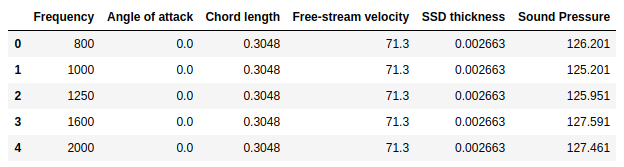
\includegraphics[scale=0.6]{img/train_head.png}
\caption{Tabla con las 5 primeras muestras del conjunto de training.}
\end{figure}

    Antes de proseguir, vamos a dividir los datos en los conjuntos de
training y test, ya que en este caso disponemos solo de un conjunto de
datos (no viene separado por defecto). Para esto, vamos a crear primero
una función que nos permita dividir los datos que tenemos en las
características (a lo que llamaremos \(\mathbf{X}\)) y las etiquetas (a
lo que llamaremos \(y\)). Una vez hecha esta separación, podremos
dividir los datos en los dos conjuntos anteriormente mencionados. Vamos
a hacer que el 80\% de los datos se quede en training y que el 20\% de
los datos esté en test. Por tanto, en resumidas cuentas, estamos
haciendo \emph{hold-out}, ya que nos quedamos con una parte de los datos
para poder estimar un E\(_{test}\) que nos permita acotar E\(_{out}\)
posteriormente. Esto tiene sus efectos negativos, como que por ejemplo
tengamos menos datos con los que entrenar y que los resultados pueden
ser un poco peores por este motivo, pero al menos tenemos una capacidad
para probar como de bueno es nuestro ajuste fuera de la muestra con la
que lo hemos entrenado.

Con esto dicho, vamos a ver como ser haría:

    \begin{Verbatim}[commandchars=\\\{\}]
{\color{incolor}In [{\color{incolor}3}]:} \PY{c+c1}{\PYZsh{} Función para dividir los datos en train y test}
        \PY{k+kn}{from} \PY{n+nn}{sklearn}\PY{n+nn}{.}\PY{n+nn}{model\PYZus{}selection} \PY{k}{import} \PY{n}{train\PYZus{}test\PYZus{}split}
        
        \PY{k}{def} \PY{n+nf}{divide\PYZus{}data\PYZus{}labels}\PY{p}{(}\PY{n}{input\PYZus{}data}\PY{p}{)}\PY{p}{:}
            \PY{l+s+sd}{\PYZdq{}\PYZdq{}\PYZdq{}}
        \PY{l+s+sd}{    Funcion que divide una muestra en los datos y las etiquetas}
        \PY{l+s+sd}{    }
        \PY{l+s+sd}{    :param input\PYZus{}data Conjunto de valores que se quieren separar}
        \PY{l+s+sd}{                      juntados en un DataFrame}
        \PY{l+s+sd}{    }
        \PY{l+s+sd}{    :return Devuelve los datos y las etiquetas}
        \PY{l+s+sd}{    \PYZdq{}\PYZdq{}\PYZdq{}}
            
            \PY{c+c1}{\PYZsh{}Obtener los valores}
            \PY{n}{values} \PY{o}{=} \PY{n}{input\PYZus{}data}\PY{o}{.}\PY{n}{values}
            
            \PY{c+c1}{\PYZsh{} Obtener datos y etiquetas}
            \PY{n}{X} \PY{o}{=} \PY{n}{values}\PY{p}{[}\PY{p}{:}\PY{p}{,} \PY{p}{:}\PY{o}{\PYZhy{}}\PY{l+m+mi}{1}\PY{p}{]}
            \PY{n}{y} \PY{o}{=} \PY{n}{values}\PY{p}{[}\PY{p}{:}\PY{p}{,} \PY{o}{\PYZhy{}}\PY{l+m+mi}{1}\PY{p}{]}
            
            \PY{k}{return} \PY{n}{X}\PY{p}{,} \PY{n}{y}
        
        \PY{c+c1}{\PYZsh{} Obtener valores X, Y}
        \PY{n}{X}\PY{p}{,} \PY{n}{y} \PY{o}{=} \PY{n}{divide\PYZus{}data\PYZus{}labels}\PY{p}{(}\PY{n}{df}\PY{p}{)}
        
        \PY{c+c1}{\PYZsh{} Dividir los datos en training y test}
        \PY{n}{X\PYZus{}train}\PY{p}{,} \PY{n}{X\PYZus{}test}\PY{p}{,} \PY{n}{y\PYZus{}train}\PY{p}{,} \PY{n}{y\PYZus{}test} \PY{o}{=} \PY{n}{train\PYZus{}test\PYZus{}split}\PY{p}{(}\PY{n}{X}\PY{p}{,} \PY{n}{y}\PY{p}{,} 
                        \PY{n}{test\PYZus{}size}\PY{o}{=}\PY{l+m+mf}{0.2}\PY{p}{,} \PY{n}{random\PYZus{}state}\PY{o}{=}\PY{l+m+mi}{1}\PY{p}{,} \PY{n}{shuffle}\PY{o}{=}\PY{k+kc}{True}\PY{p}{)}
\end{Verbatim}

    Con los datos ya cargados y divididos en los conjuntos de training y
test, vamos a obtener cierta información sobre éstos. En problemas de
este tipo nos interesa conocer por ejemplo si en ciertos casos faltan
datos (no se ha podido obtener información sobre todos los atributos
debido a que es imposible hacerlo, han habido errores a la hora de
tomarlos o no se disponía de las herramientas necesarias), el número de
valores distintos, los rangos de los datos (valores mínimos y máximos
para cada atributo), si existe algún tipo de correlación entre las
variables, etc.

Vamos a comenzar estudiando primero las características más simples,
para adentrarnos luego en el estudio de la correlación. Empecemos
mirando información del conjunto training\footnote{El módulo que se ha utilizado para obtener la información resumida no viene instalado por defecto en el entorno de \textit{conda} y no se puede instalar en éste. Se puede instalar mediante pip, pero como tal, no se encuentra disponible para \textit{conda}. Por tanto, al no poder utilizarlo en Spyder, no se incluirá esta funcionalidad en el código entregado.}:

    \begin{Verbatim}[commandchars=\\\{\}]
{\color{incolor}In [{\color{incolor}4}]:} \PY{c+c1}{\PYZsh{} Clase para mostrar información de DataFrames resumida}
        \PY{k+kn}{from} \PY{n+nn}{pandas\PYZus{}summary} \PY{k}{import} \PY{n}{DataFrameSummary}
        \PY{k+kn}{from} \PY{n+nn}{IPython}\PY{n+nn}{.}\PY{n+nn}{core}\PY{n+nn}{.}\PY{n+nn}{display} \PY{k}{import} \PY{n}{display}
        
        \PY{c+c1}{\PYZsh{} Crear información resumida sobre los datos de training}
        \PY{n}{train\PYZus{}df} \PY{o}{=} \PY{n}{pd}\PY{o}{.}\PY{n}{DataFrame}\PY{p}{(}\PY{n}{columns}\PY{o}{=}\PY{n}{column\PYZus{}names}\PY{p}{,}
                                \PY{n}{data}\PY{o}{=}\PY{n}{np}\PY{o}{.}\PY{n}{c\PYZus{}}\PY{p}{[}\PY{n}{X\PYZus{}train}\PY{p}{,} \PY{n}{y\PYZus{}train}\PY{p}{]}\PY{p}{)}
        
        \PY{c+c1}{\PYZsh{} Crear un DataFrame de resumen y mostrarlo}
        \PY{n}{train\PYZus{}sum} \PY{o}{=} \PY{n}{DataFrameSummary}\PY{p}{(}\PY{n}{train\PYZus{}df}\PY{p}{)}\PY{o}{.}\PY{n}{summary}\PY{p}{(}\PY{p}{)}
        \PY{n}{display}\PY{p}{(}\PY{n}{train\PYZus{}sum}\PY{p}{)}
\end{Verbatim}

\begin{figure}[H]
\centering
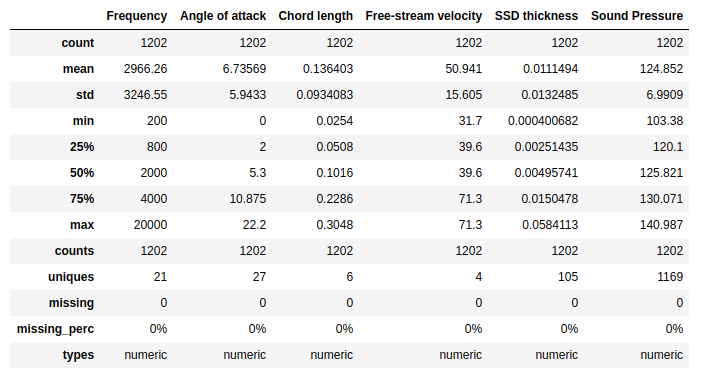
\includegraphics[scale=0.55]{img/train_summary.png}
\caption{Tabla que contiene el resumen de los datos de training.}
\end{figure}

    Aquí podemos ver que para ninguna de las variables faltan datos, lo cuál
nos ahorra tiempo extra de procesado en el que tendríamos que insertar
valores a partir de algún valor estadístico (valores medios, por
ejemplo).

También podemos ver información sobre como varían los datos, tanto los
de entrada como los de salida. Vemos que, por ejemplo,
\textbf{Frequency} es una característica que varía mucho, ya que tiene
unos valores mínimos y máximos muy dispares, además de tener una
desviación típica muy elevada. Posiblemente este atributo contenga
\emph{outliers}, pero al no disponer de demasiados datos, y al ser tan
pocos los posibles valores anómalos, no merece la pena intentar
eliminarlos. Observando el resto de características, nos encontramos con
unos valores que varían menos y cuyos rangos de valores más pequeño. Lo
sorprendente es que, para los datos de entrada, tenemos que hay muy
pocos valores únicos (no repetidos). Esto se puede deber a que no se han
medido los valores con suficiente precisión o a que no exista una
verdadera variabilidad entre ellos. Para los datos de salida, en cambio,
nos encontramos que hay un montón de valores distintos. Esto es normal,
ya que, al ser valores reales, hay muchos posibles valores. De aquí
podemos concluir que, a pesar de que nos encontremos ante un problema
con variable reales, parece que los valores que toman las variables de
entrada están discretizados, es decir, que no son exactamente contínuos.

Pasemos ahora a analizar el conjunto de datos de entrenamiento. Para
obtener suficiente información, vamos a fijarnos solo en valores únicos
y si faltan datos, teniendo en cuenta que nunca debemos obtener
información completa sobre los datos de test, ya que se supone que nunca
serán conocidos y que nunca deberíamos verlos. A continuación, podemos
ver esta información:

    \begin{Verbatim}[commandchars=\\\{\}]
{\color{incolor}In [{\color{incolor}5}]:} \PY{c+c1}{\PYZsh{} Crear DataFrame con los datos de test}
        \PY{n}{test\PYZus{}df} \PY{o}{=} \PY{n}{pd}\PY{o}{.}\PY{n}{DataFrame}\PY{p}{(}\PY{n}{columns}\PY{o}{=}\PY{n}{column\PYZus{}names}\PY{p}{,}
                               \PY{n}{data}\PY{o}{=}\PY{n}{np}\PY{o}{.}\PY{n}{c\PYZus{}}\PY{p}{[}\PY{n}{X\PYZus{}test}\PY{p}{,} \PY{n}{y\PYZus{}test}\PY{p}{]}\PY{p}{)}
        
        \PY{c+c1}{\PYZsh{} Crear un DataFrame resumen y mostrar algunos}
        \PY{c+c1}{\PYZsh{} valores estadísticos}
        \PY{n}{test\PYZus{}sum} \PY{o}{=} \PY{n}{DataFrameSummary}\PY{p}{(}\PY{n}{test\PYZus{}df}\PY{p}{)}\PY{o}{.}\PY{n}{columns\PYZus{}stats}
        \PY{n}{display}\PY{p}{(}\PY{n}{test\PYZus{}sum}\PY{p}{)}
\end{Verbatim}

\begin{figure}[H]
\centering
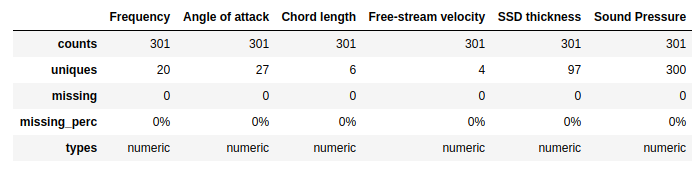
\includegraphics[scale=0.55]{img/test_summary.png}
\caption{Tabla que contiene el resumen de los datos de test.}
\end{figure}

Como se puede ver, el número de valores únicos, para las variables de
entrada, son muy próximos a los que teníamos anteriormente. En el caso
de los valores de salida, podemos observar que hay mucha diversidad. Y,
finalmente, como punto positivo, podemos ver que en ninguna de las
muestras faltan datos.

Una vez hecho este pequeño análisis, pasemos a observar ahora la
correlación entre las variables. Vamos a intentar obtener, para cada una
de las variables (tanto las de entrada como las de salida) el
coeficiente de correlación de Pearson. El resultado se puede ver a
continuación:

    \begin{Verbatim}[commandchars=\\\{\}]
{\color{incolor}In [{\color{incolor}6}]:} \PY{c+c1}{\PYZsh{} Obtener gráfica de correlación de Pearson}
        \PY{n}{corr} \PY{o}{=} \PY{n}{train\PYZus{}df}\PY{o}{.}\PY{n}{corr}\PY{p}{(}\PY{p}{)}
        \PY{n}{corr}\PY{o}{.}\PY{n}{style}\PY{o}{.}\PY{n}{background\PYZus{}gradient}\PY{p}{(}\PY{n}{cmap}\PY{o}{=}\PY{l+s+s1}{\PYZsq{}}\PY{l+s+s1}{Spectral}\PY{l+s+s1}{\PYZsq{}}\PY{p}{)}
\end{Verbatim}

\begin{figure}[H]
\centering
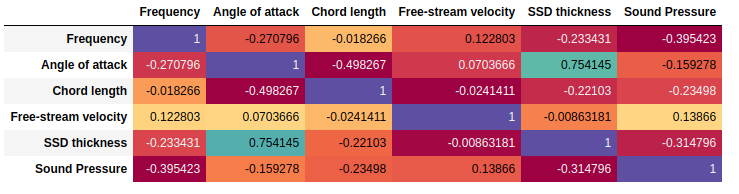
\includegraphics[scale=0.5]{img/tabla_correlacion.png}
\caption{Tabla con los coeficientes de Pearson para cada par de variables.}
\end{figure}
            
    Se puede ver que, en general, no existe una correlación entre la mayoría
de las características. Sin embargo, sí que destacan dos casos, uno más
que el otro. El primer caso es la relación que existe entre la
característica \textbf{SSD thickness} y la característica \textbf{Angle
of attack}. Estas dos características tienen una coeficiente de
correlación de Pearson de \(0.75\), valor que es muy próximo a \(1\).
Por tanto, podemos decir que existe cierta correlación entre ellas, ya
que el crecimiento de una influirá en el crecimiento de la otra. Sin
embargo, como el valor del coeficiente de Pearson no es 1, no podríamos
asegurar con absoluta confianza que las 2 características estén
correlacionadas, y que por tanto, sería necesario eliminar una de ellas.
El segundo caso es \textbf{Chord length} y \textbf{Angle of attack}.
Aquí lo que sucede es que el coeficiente de correlación de Pearson tiene
un valor de aproximadamente \(-0.5\). Con lo cuál, a pesar de que existe
cierta correlación negativa entre las dos variables (cuando crezca una,
la otra decrecerá), no podríamos afirmar con un 100\% de confianza que
estén totalmente correlacionadas, ya que el valor del coeficiente está
en un punto medio.

Para tener una mejor visión de todo lo que se acaba a discutir, vamos a
ver un conjunto de gráficas en las que se pueden ver los valores de
todas las variables dos a dos (es decir, se muestran gráficas para
mostrar como cambia cada par de variables, que pueden ser tanto las
características como la etiqueta de salida). Esto se puede ver a
continuación:

    \begin{Verbatim}[commandchars=\\\{\}]
{\color{incolor}In [{\color{incolor}7}]:} \PY{c+c1}{\PYZsh{} Módulo avanzado para dibujar gráficas}
        \PY{k+kn}{import} \PY{n+nn}{seaborn} \PY{k}{as} \PY{n+nn}{sns}
        
        \PY{c+c1}{\PYZsh{} Crear pares de plots para cada 2 atributos}
        \PY{c+c1}{\PYZsh{} También se incluyen las etiquetas}
        \PY{n}{sns}\PY{o}{.}\PY{n}{set\PYZus{}style}\PY{p}{(}\PY{l+s+s2}{\PYZdq{}}\PY{l+s+s2}{whitegrid}\PY{l+s+s2}{\PYZdq{}}\PY{p}{)}
        \PY{n}{sns}\PY{o}{.}\PY{n}{pairplot}\PY{p}{(}\PY{n}{train\PYZus{}df}\PY{p}{)}
        
        \PY{c+c1}{\PYZsh{} Mostrar el plot}
        \PY{n}{plt}\PY{o}{.}\PY{n}{show}\PY{p}{(}\PY{p}{)}
\end{Verbatim}

\newpage

\section{\textsc{Problema de Clasificación}}

\newpage

\begin{thebibliography}{5}

\bibitem{nombre-referencia}
Texto referencia
\\\url{https://url.referencia.com}

\end{thebibliography}

\end{document}

